% Template for ICASSP-2013 paper; to be used with:
%          spconf.sty  - ICASSP/ICIP LaTeX style file, and
%          IEEEbib.bst - IEEE bibliography style file.
% --------------------------------------------------------------------------
\documentclass{article}
\usepackage{spconf,amsmath,graphicx}
\usepackage{graphicx}
\usepackage{cite}
\usepackage{url}
\usepackage{hyperref}
\usepackage{cleveref}
\usepackage{booktabs}
\usepackage{brian}

% Title.
% ------
\title{Learning to segment songs with ordinal linear discriminant analysis}
%
% Single address.
% ---------------
% \name{Author Names\thanks{Thanks to XYZ agency for funding.}}
% \address{Author Affiliations}
%
% For example:
% ------------
%\address{School\\
%   Department\\
%   Address}
%
% Two addresses (uncomment and modify for two-address case).
% ----------------------------------------------------------
\twoauthors%
 {Brian McFee}{ Center for Jazz Studies\\
      Columbia University\\
  \texttt{brm2132@columbia.edu}}%
 {Daniel P.W. Ellis}{
  LabROSA, Department of Electrical Engineering\\
      Columbia University\\
  \texttt{dpwe@columbia.edu}}
%
\begin{document}
%\ninept
%
\maketitle
%
\begin{abstract}
This paper describes a supervised learning algorithm which optimizes a feature representation for temporally constrained clustering. 
The proposed method is applied to music segmentation, in which a song is partitioned into functional or
locally homogeneous segments (\eg, verse, chorus or solo).  Experimental results on the SALAMI and Beatles corpora demonstrate
that the proposed method efficiently integrates disparate feature modalities, and improves segmentation accuracy.
\end{abstract}
%
\begin{keywords}
Music information retrieval, automatic segmentation, supervised learning
\end{keywords}
%
\section{Introduction}
\label{sec:intro}


\subsection{Our contributions}
Our primary contribution in this work is the ordinal linear discriminant analysis (OLDA) technique to learn a 
feature transformation which is optimized for musical segmentation, or more generally, time-series clustering.
As a secondary contribution, we propose a latent structural repetition descriptor, which facilitates learning and
generalization across multiple examples when using self-similarity features.

\subsection{Related work}
\label{sec:related}

The core segmentation algorithm we use is most similar to the constrained clustering method developed by Levy and
Sandler~\cite{levy2008structural}, which incorporated sequential consistency constraints to a hidden Markov model over
segment transitions. The method proposed here is much simpler, and uses a sequentially constrained agglomerative
clustering algorithm to produce a hierarchical segmentation over the entire track.  Because the
resulting segmentation is hierarchical, the number of segments need not be specified in advance.

The proposed latent structural repetition features are adapted from the work of Serr\`{a}
\etal~\cite{serra2012unsupervised}. While qualitatively similar, we apply different filtering and
beat synchronization techniques to better preserve segment boundaries. 
In addition to chord sequence repetitions, our method includes timbre repetitions, as well as 
localized timbre and pitch features, and timing information.

\section{Music segmentation}
\label{sec:features}
Partitioning a song into \emph{segments} is a somewhat ill-posed task, and the criteria for deciding what is or
is not a segment may vary across genres or styles.  Pop music relies heavily on a verse/chorus structure, while jazz
may more naturally be structured by changing instrumentation (\ie, which player is currently soloing).  
The former case is well characterized by detecting repeated chord sequences, and the latter is better modeled
by finding sequences of locally homogenous timbre.

We follow the strategy used by Serr\`{a} \etal, which first converts global structural (repetitions) into
local feature vectors, and then segments by detecting changes in the resulting time-series. 
When combined with the learning algorithm described in \Cref{sec:olda}, this framework facilitates the 
combination of global and local information to simultaneously capture both high-level structure and low-level 
consistency.

\subsection{Latent structural repetition}
\Cref{fig:rep} outlines our approach for computing structural repetition features from audio, which is adapted from
Serr\`{a} \etal~\cite{serra2012unsupervised}.  First, we extract beat-synchronous features (\eg, MFCCs or chroma) 
from the signal, and build a binary self-similarity matrix by linking each beat to its nearest neighbors in feature
space (\cref{fig:rep}, left). With beat-synchronous features, repeated sections appear as diagonals in the self-similarity
matrix. To easily detect repeated sections, the self-similarity matrix is skewed by shifting the $i$th column down by $i$ rows
(\cref{fig:rep}, second subplot), thus converting diagonals into horizontals.

Using nearest-neighbor linkage to compute the self-similarity matrix results in spurious links and skipped connections. 
Serr\`{a}~\etal{} resolve this by convolving with a Gaussian filter, which effectively suppresses noise, but also blurs
segment boundaries. Instead, we propose to use a horizontal median filter, which (for odd window length) produces a binary matrix,
suppresses links which do not belong to long sequences of repetitions, and fills in skipped conections (\cref{fig:rep}, third
subplot). Because median filtering preserves edges, we may expect more precise boundary detection.

Let $R \in \R^{2t \times t}$ denote the median-filtered, skewed self-similarity matrix over $t$ beats.  
Note that different songs have different durations, so the dimensionality of $R$ changes from one song to this. 
This makes it difficult to directly model and generalize across collections of songs.
However, methods which depend on distances between column-vectors ${\|R_{\cdot, i} - R_{\cdot, j}\|}$ --- 
\eg, Euclidean clustering or novelty curve peak-picking --- are invariant to unitary transformations.

Rather than use $R$ directly as a feature matrix, we propose to use \emph{latent structural repetition} features, which compress each
any song's $R$ matrix to a fixed-dimension representation.  Let $R = U\Sigma V\trans$ denote the singular value decomposition of $R$,
with (descending) singular values $\sigma_i$. The latent structural repetition feature (\cref{fig:rep}, right) is defined as the 
matrix $L$:
\begin{equation}
L \defeq \sigma_1^{-1} U\trans R = \sigma_1^{-1} \Sigma V\trans.\label{eq:latent-rep}
\end{equation}
Truncating $L$ to $d < 2t$ rows preserves the most important factors, and normalizing by $\sigma_1$ ensures that
features maintain the same relative magnitude independent of track duration.  As depicted in \Cref{fig:rep}, small values of $d$
suffice to capture high-level structure: in the given example, the key structural components are indicated by the value of the first
factor.

\begin{figure*}[t]
\centering%
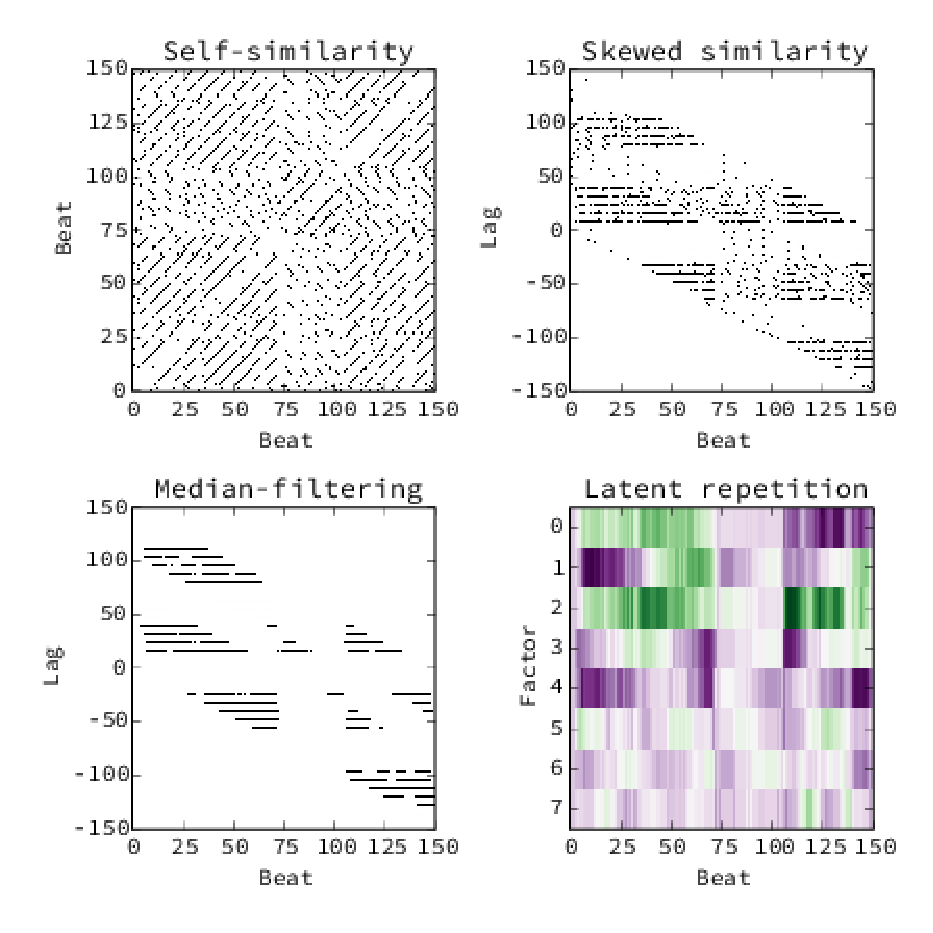
\includegraphics[width=\textwidth]{figs/rep}
\vspace{-2\baselineskip}
\caption{Repetition features derived from \emph{Tupac Shakur -- Trapped}. 
From left to right: a binary self-similarity ($k$-nearest-neighbor) 
matrix over beats; 
the time-lag transformation of the self-similarity matrix; 
the result of the horizontal median filter;
the derived 8-dimensional latent factor representation (best viewed in color).\label{fig:rep}}
\end{figure*}

\subsection{Constrained agglomerative clustering}
\label{sec:clustering}
Given a feature matrix $X \in \R^{D\times t}$, we produce a hierarchical clustering of the columns of $X$ by using the
linkage-constrained variant of Ward's agglomerative clustering algorithm~\cite{ward1963hierarchical} as implemented in
\texttt{scikit-learn}~\cite{pedregosa2011scikit}.  Specifically, for each column $i$, linkage constraints are generated
for $(i-1, i)$ and $(i, i+1)$, so the linkage graph forms a chain.  Starting from $t$ clusters (each column of $X$), the 
algorithm then iteratively merges the two closest (feasible) clusters until only one remains.
Due to the chain graph constraint, the full hierarchy is computed after at most $\Oh(t)$ merge operations. Each merge operation
takes time $\Oh(D + \log t)$ (to compute distance and manage a priority queue), so the algorithm runs in $\Oh(tD + t\log t)$ time.
For the typical case of $D > \log t$, the cost of clustering is dominated by the cost of computing the feature matrix $X$.

\subsection{Choosing the number of segments}
The hierarchical clustering produces segmentations for all numbers of segments $1 \leq k \leq t$.  While a multi-scale view can 
be useful in some scenarios --- such as interactive data exploration --- standard evaluations rely on choosing a particular value 
of $k$. To select $k$ automatically, we compute the cost (quantization error) of each pruning within a plausible bounded range 
$k_{\min} \leq k \leq k_{\max}$.  The bounds are determined dynamically by assuming average minimum and maximum segment duration 
of 10s and 45s.  AIC correction~\cite{akaike1973information} is then applied to each pruning (assuming a spherical Gaussian
model for each segment), and the best value of $k$ is chosen to minimize the AIC-corrected cost.

\subsection{Multiple features}
Structural repetition features are most commonly used to detect repeated chord sequences, but the idea is general enough to
support any kind of feature descriptor.  We aggregate several types of feature descriptors for each beat:
\begin{description}\addtolength{\itemsep}{-0.5\baselineskip}%
\item[MFCC]   Beat-synchronous (mean) Mel-frequency cepstral coefficients and their latent repetitions;
\item[Chroma] Beat-synchronous (median) chroma vectors and their latent repetitions; and
\item[Time]   Beat time-stamps (seconds), (duration) normalized beat time-stamps, beat indices ($1, 2, \ldots, t$), 
and normalized beat indices ($1/t, 2/t, \ldots, 1.0$).
\end{description}
The MFCC features roughly capture local timbre and timbre sequences. The chroma features capture local pitch similarity and pitch
sequences. Finally, the time features act as an implicit quadratic regularization on segment durations, and encourages
balanced segmentations.

All features can be stacked together into a single feature matrix $X \in \R^{D\times t}$, and clustered via the method described
above. However, the relative magnitude and importance of each feature is not calibrated to produce optimal clusterings. 

\section{Ordinal linear discriminant analysis}
\label{sec:olda}
To improve the feature representation for clustering, we propose a simple adaptation of Fisher's linear discriminant
analysis (FDA)~\cite{fisher1936use}.  In its multi-class form, FDA takes as input a labeled collection of data $x_i \in \R^D$
and class labels $y_i \in \{1,2,\ldots, C\}$, and produces a linear transformation $W \in \R^{D\times D}$ that simultaneously 
maximizes the distance between class centroids, and minimizes the variance of each class 
individually~\cite{fukunaga1990introduction}. This is accomplished by solving the following optimization:
\begin{equation}
W \defeq \argmax_W \trace\left( {(W\trans A_\text{W} W)}^{-1} W\trans A_\text{B} W \right) \label{eq:fda},
\end{equation}
where $A_\text{W}$ and $A_\text{B}$ are the \emph{within-} and \emph{between}-class scatter matrices:
\begin{align*}
A_\text{W} & \defeq \sum_c \sum_{i : y_i = c} (x_i - \mu_c)(x_i - \mu_c)\trans\\
A_\text{B} & \defeq \sum_c n_c (\mu_c - \mu)(\mu_c - \mu)\trans,
\end{align*}
$\mu$ denotes the mean across all classes, $\mu_c$ is the mean of class $c$, and $n_c$ denotes the number of examples in class $c$.
\Cref{eq:fda} can be efficiently solved as a generalized eigenvalue problem over the two scatter matrices $(A_\text{B},
A_\text{W})$~\cite{de2005eigenproblems}.

Class labels can be synthesized from segments on an annotated training song, so that the columns of $X$ belonging to the first 
segment are assigned to class 1, the second segment to class 2, and so on.
However, interpreting each segment as a distinct class could result in a repeated verse being treated as two distinct classes which 
cannot be separated. 
A more serious problem with this formulation is that it is unclear how to generalize across multiple songs, as it would result in
FDA attempting to separate segments from different songs, which is somewhat meaningless for the single-song segmentation task.

Now, note that due to linkage constraints, the agglomerative clustering algorithm (\cref{sec:clustering}) only considers merge 
operations over adjacent segments $(c, c+1)$. This motivates a relaxed FDA problem which only attempts to separate adjacent
segments.  This is accomplished by replacing the between-class scatter matrix $A_B$ with the resulting \emph{ordinal scatter matrix}:
\begin{align*}
A_\text{O} &\defeq \sum_{c < C} n_c (\mu_c - \mu_{c+}) (\mu_c - \mu_{c+})\trans\\
\mu_{c+} &\defeq \frac{n_c \mu_c + n_{c+1} \mu_{c+1} }{n_c + n_{c+1}}.
\end{align*}

Because scatter matrices are accumulated linearly, it is also straightforward to generalize this across multiple training songs
by summing their individual contributions.  Finally, because $A_\text{O}$ may be rank-degenerate, we include a smoothing parameter
$\lambda > 0$.  The OLDA optimization takes the form:
\begin{equation}
W \defeq \argmax_W \trace\left( {(W\trans (A_\text{W} + \lambda I) W)}^{-1} W\trans A_\text{O} W \right) \label{eq:olda},
\end{equation}
which again can be solved efficiently as a generalized eigenvalue problem over the matrix pair 
$(A_\text{O}, A_\text{W} + \lambda I)$.

After learning $W$, the feature matrix $X$ for a previously unseen song is transformed via $X \mapsto W\trans X$, and then 
given as input to the clustering algorithm described in \Cref{sec:clustering}.

\section{Evaluation}
\label{sec:eval}
All proposed methods are implemented in Python with the \texttt{librosa} package.\footnote{Source code is
available at \url{https://github.com/bmcfee/olda}.}  
All signals were downsampled to 22KHz mono, and analyzed with a 93ms window and 3ms hop.  MFCCs are generated from 128 Mel bands
with an 8KHz cutoff. We take 32 MFCCs and 12 chroma bins; repetition features are calculated with $2\sqrt{t}$ nearest neighbors,
median-filtered with a window width of 7, and projected to 32 dimensions each.  Including the four time-stamp features, the combined
representation has dimension $D=112$. Beat tracking was done using the \emph{med-full} method described in~\cite{mcfee2014beat}.

\subsection{Data and metrics}
To evaluate the proposed methods, we evaluate predicted segmentations on two publicly available datasets:
\begin{description}\addtolength{\itemsep}{-0.25\baselineskip}%
\item[Beatles-ISO] 179 songs by the Beatles~\cite{harte2010towards,isophonicsbeatles}, and
\item[SALAMI-free] 253 songs from the SALAMI dataset~\cite{smith2011design} which are freely available on the 
Internet Archive~\cite{nieto2013convex}.
\end{description}
Both datasets provide labels for each annotated segment (\eg, \emph{verse} or \emph{intro}), but we ignore these
labels in this set of experiments. Compared to the Beatles corpus, SALAMI has much more diversity of style, genre, 
instrumentation, and artists, and is therefore a more challenging dataset.

On both datasets, we compare to the method of Serr\`{a} \etal~\cite{serra2012unsupervised}, which achieved the
highest performance in the 2012 MIREX structural segmentation evaluation~\cite{Downie2008}.
On SALAMI-Free, we include previously published results for the C-NMF~\cite{nieto2013convex} and SI-LPCA~\cite{weiss2011unsupervised}.

For both datasets, we evaluate the unweighted feature representation (\emph{Unweighted}), FDA optimization (using the
one-class-per-segment approach described in \Cref{sec:olda}), and the OLDA-optimized
representation. To ensure fairness of evaluation, the FDA and OLDA models used on the Beatles-ISO were trained using only
SALAMI-free data, and vice versa.  FDA\footnote{We apply the same regularization strategy to FDA as in OLDA, $A_\text{W} + \lambda
I$.} and OLDA models were trained by running the entire segmentation algorithm for
$\lambda \in \{10^0, 10^1, \dots, 10^7\}$, and choosing the value which achieved the highest mean $S_F$ score (see below) on 
the training set.


We report the following standard segmentation metrics:
\footnote{For a detailed description of segmentation metrics, see~\cite{mirexstructure}.}
\begin{description}\addtolength{\itemsep}{-0.25\baselineskip}%
\item[Boundary retrieval] Precision, recall, and F-measure at both 0.5s and 3s resolution,
\item[Normalized conditional entropy] (NCE) Over- and under-segmentation scores $S_O$ and $S_U$, and their harmonic
mean $S_F$, and
\item[Frame clustering] Precision ($P_C$), recall ($R_C$), and F-measure ($F_C$) of detecting whether any two frames 
belong to the same segment.
\end{description}
Note that boundary retrieval and frame clustering metrics are highly sensitive to changes in the number of
predicted segments, upon which multiple human annotators often disagree for the same track. 
The NCE metrics are designed to be fairly robust to changes in segmentation granularity.
Following MIREX practice, frames are sampled at a frequency of 10Hz for the NCE and frame clustering metrics. 


\subsection{Results}
\label{sec:results}
\begin{table*}
\centering
\caption{Segmentation results. Best scores are indicated in bold; significance is assessed with a Bonferroni-corrected Wilcoxon
signed-rank test with $p=0.05$. C-NMF and SI-LPCA scores are quoted from~\cite{nieto2013convex}.\label{tab:results}}
\footnotesize
\begin{tabular}{lrrrrrrrrrrrr}
% \bottomrule%
\multicolumn{13}{c}{Beatles-ISO}\\
\toprule%
Algorithm   &   $P_{0.5s}$ & $R_{0.5s}$ & $F_{0.5s}$ & $P_{3s}$     & $R_{3s}$  & $F_{3s}$   & $S_O$ & $S_U$ & $S_F$ & $P_C$& $R_C$& $F_C$\\
\hline
Unweighted  &   \textbf{0.446} & 0.390 & 0.408 & 0.704   & 0.603 & 0.640 & \textbf{0.842} & 0.755 & 0.791 & \textbf{0.780} & 0.613 & 0.668\\
FDA         &   \textbf{0.455} & 0.416 & \textbf{0.427} & 0.688 & 0.620 & 0.642 & \textbf{0.839} & 0.778 & 0.802 & \textbf{0.774} & 0.653 & 0.691\\
OLDA        &   0.438 & \textbf{0.447} & \textbf{0.434} & 0.685   & 0.680 & 0.670 & 0.828 & 0.808 & 0.813 & 0.744 & 0.686 & 0.694\\
\hline
SMGA~\hfill\cite{serra2012unsupervised}
            &   0.358 & 0.393 & 0.370 & \textbf{0.769}   & \textbf{0.808} & \textbf{0.780} & 0.811 & \textbf{0.858} & \textbf{0.829} & 0.702 & \textbf{0.798} &
            \textbf{0.729}\\
\toprule%
\multicolumn{13}{c}{SALAMI-free}\\
\toprule%
Unweighted  & 0.400 & 0.364 & 0.372 & 0.610 & 0.557 & 0.570 & 0.812 & 0.795 & 0.794 & 0.666 & 0.652 & 0.626\\
FDA     &  \textbf{0.492} & 0.349 & \textbf{0.397} & \textbf{0.694} & 0.511 & 0.574 & \textbf{0.849} & 0.729 & 0.771 &
\textbf{0.751} & 0.566 & 0.603\\
OLDA    &  0.406 & \textbf{0.407} & \textbf{0.396} & 0.610 & 0.611 & \textbf{0.597} & 0.804 & 0.829 & \textbf{0.808} & 0.640 & 0.707 & \textbf{0.640}\\
\hline
SMGA~\hfill\cite{serra2012unsupervised}
        & 0.209 & 0.360 & 0.256 & 0.512 & \textbf{0.733} & \textbf{0.589} & 0.714 & \textbf{0.895} & 0.786 & 0.448 & \textbf{0.822} & 0.550\\
C-NMF~\hfill\cite{nieto2013convex}            
        & -- & -- & -- & 0.430 & 0.523 & 0.451 & -- & -- & -- & -- & -- & -- \\
SI-PLCA~\hfill\cite{weiss2011unsupervised}    
        & -- & -- & -- & 0.195 & 0.461 & 0.256 & -- & -- & -- & -- & -- & -- \\  
\bottomrule%
\end{tabular}
\end{table*}

% \begin{figure}
% \flushright%
% 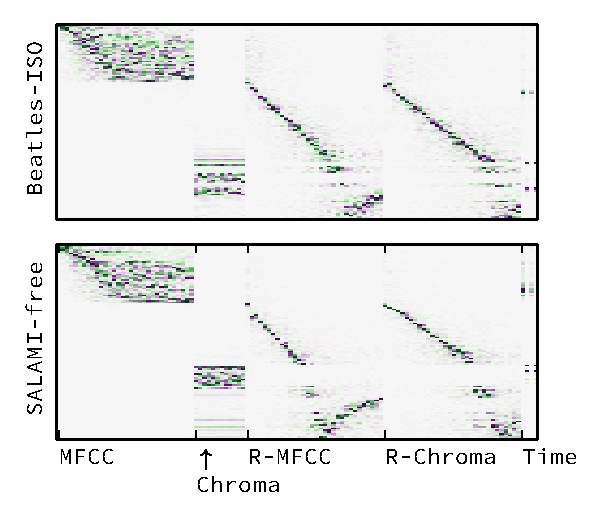
\includegraphics[width=\columnwidth]{figs/w}%
% \vspace{-\baselineskip}%
% \caption{OLDA models $W\trans$ learned on Beatles-ISO and SALAMI-free. Each row corresponds to a direction, 
% and they are ordered by decreasing importance from top to bottom.\label{fig:w}}
% \end{figure}

% \begin{figure}
% \flushright%
% 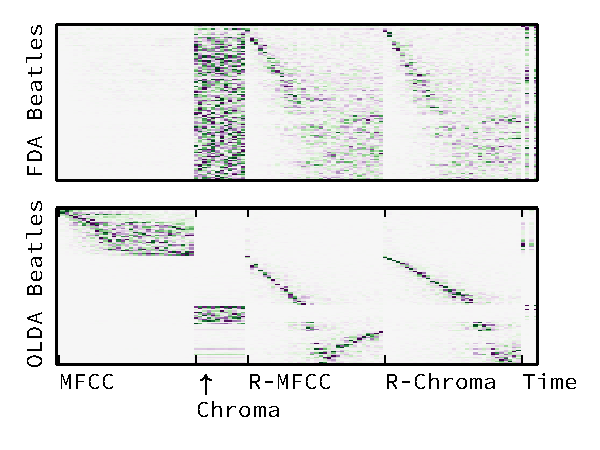
\includegraphics[width=\columnwidth]{figs/fda-vs-olda}%
% \vspace{-\baselineskip}%
% \caption{FDA and OLDA models $W\trans$ learned on Beatles-ISO. Each row corresponds to a direction, 
% and they are ordered by decreasing importance from top to bottom.\label{fig:fda-vs-olda}}
% \end{figure}

\Cref{tab:results} list the results for the Beatles-ISO and SALAMI-free.
In \Cref{tab:results} (top), the SMGA method performs best on the majority of metrics,\footnote{We
note that the SMGA parameters were optimized to perform well on this set (listed as
Beatles-B)~\cite{serra2012unsupervised}.}
however, the scores on the NCE metrics ($S_O, S_U, S_F$) are roughly comparable between SMGA and OLDA ($S_F$ of 0.829
and 0.813, respectively). 
This suggests that SMGA and the proposed methods are producing segmentations of comparable quality, but 
different levels of granularity.
However, both the unweighted and OLDA models achieve much higher accuracy for boundary detection at 0.5s resolution,
indicating that the proposed features are better at preserving clean segment boundaries.  

On SALAMI-free (\cref{tab:results}, bottom), the trends are qualitatively similar as in Beatles-ISO, but the OLDA
model achieves the largest improvement on the combined F-scores. This is likely due to the proposed model's
ability to incorporate disparate feature types (timbre, pitch, and time), whereas the SMGA and C-NMF models are
limited to using only pitch. 
Because SALAMI-free includes a wider variety of styles and instrumentations than the Beatles-ISO set, 
timbre can be an important cue for detecting salient change-points.

In both datasets, OLDA training generally provides substantial improvements in accuracy over the unweighted model. 
The FDA models tend to improve precision, but often reduce recall.
% \Cref{fig:fda-vs-olda} illustrates the transformation matrices $W$ learned by FDA and OLDA on the Beatles-ISO data.  

% The fact that the model parameters were transferred across datasets suggests some degree of universality of the
% learned transformation.  \Cref{fig:w} illustrates the transformation matrices $W$ learned on each dataset. Both
% transformations exhibit qualitatively similar block structure, and place most of the mass on the MFCC components
% (upper-left blocks) while suppressing chroma and placing intermediate weight on the repetition features.



\section{Conclusion}
\label{sec:conclusion}


\bibliographystyle{IEEEbib}
\bibliography{refs}

\end{document}
